\section{Related Work - Activity Forecasting}

%\begin{frame}
%	\frametitle{Related Work}
%	\framesubtitle{Human Activity Classification and Activity Recognition}
%	
%	\vspace{0.4cm}
%	
%	\begin{columns}[T]
%		\column{.55\textwidth}
%		
%		\vspace{0.2cm}
%		
%		\begin{itemize}
%			\item \textbf{Nascimento {et al.} \cite{Nascimento10}:} recognise pedestrian trajectories in
%				  video sequences, in a surveillance context
%			
%			\vspace{1.2cm}
%			
%			\item \textbf{Veloso {et al.} \cite{Vail07}:} discriminatively trained Conditional Random
%				  Fields for activity recognition
%		\end{itemize}
%		
%		\column{.5\textwidth}
%		
%		\centering
%		\begin{tikzpicture}
%			\node at (1.42,0) [draw=black,ultra thick,inner sep=0pt]
%			{
%				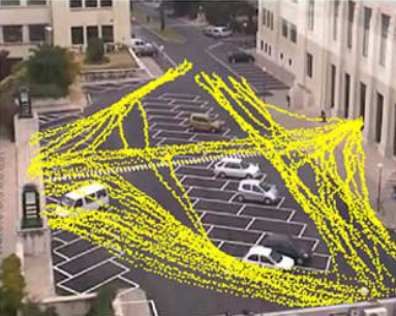
\includegraphics[height=2.2cm]{Figures/Nascimento-1}
%			};
%			\node at (-1.42,0) [draw=black,ultra thick,inner sep=0pt]
%			{
%				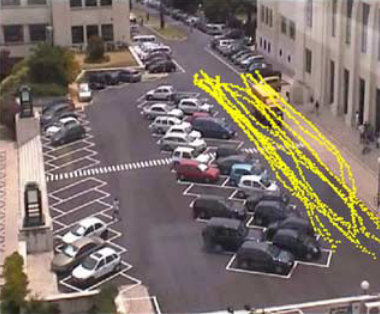
\includegraphics[height=2.2cm]{Figures/Nascimento-2}
%			};
%			\node at (0,-2.8) [draw=black,ultra thick,inner sep=0pt]
%			{
%				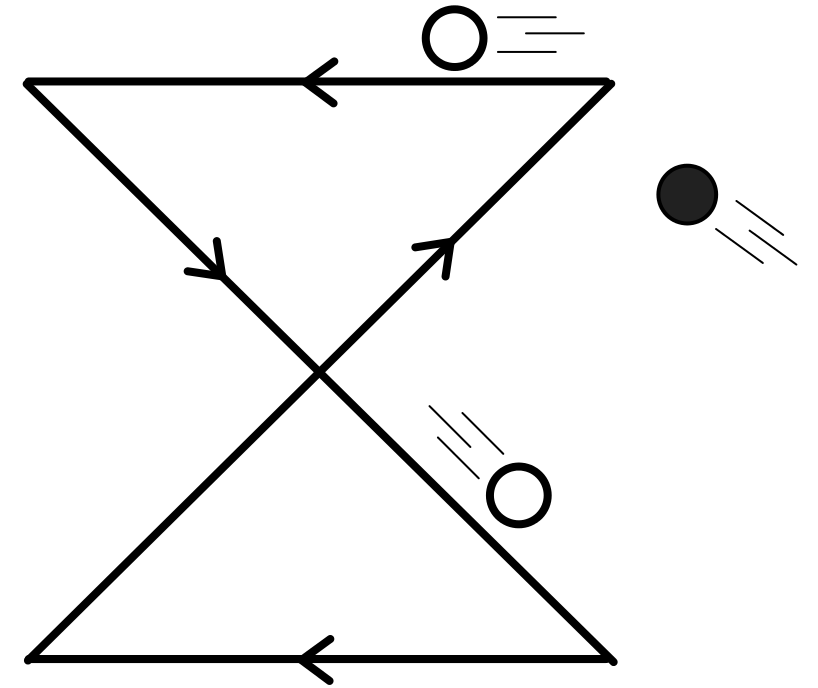
\includegraphics[width=3.6cm]{Figures/Veloso}
%			};
%		\end{tikzpicture}
%	\end{columns}
%	
%	\vspace{0.47cm}
%	
%	\tiny
%	
%	\cite{Nascimento10} J. C. Nascimento \emph{et al.}, ``Trajectory classification using switched
%	dynamical hidden Markov models'', Image Processing, 2010
%	
%	\vspace{-0.17cm}
%	
%	\cite{Vail07} D. L. Vail \emph{et al.}, ``Conditional random fields for activity recognition'',
%	AAMAS, 2007
%\end{frame}

\begin{frame}
	\frametitle{Related Work}
	\framesubtitle{Activity Forecasting through Semantic Mapping}
	
	\vspace{0.33cm}
	
	\large
	
	\textbf{Ziebart \emph{et al.} \cite{Kitani12}} propose a method for activity forecasting by
	combining:
	
	\begin{itemize}
		\item Semantic scene understanding
		\vspace{0.05cm}
		\item Inverse Optimal Control
	\end{itemize}
	
	\vspace{-0.2cm}
	
	\begin{center}
		\begin{tikzpicture}
			\node at (0,0) [draw=white,ultra thick,inner sep=0pt]
			{
				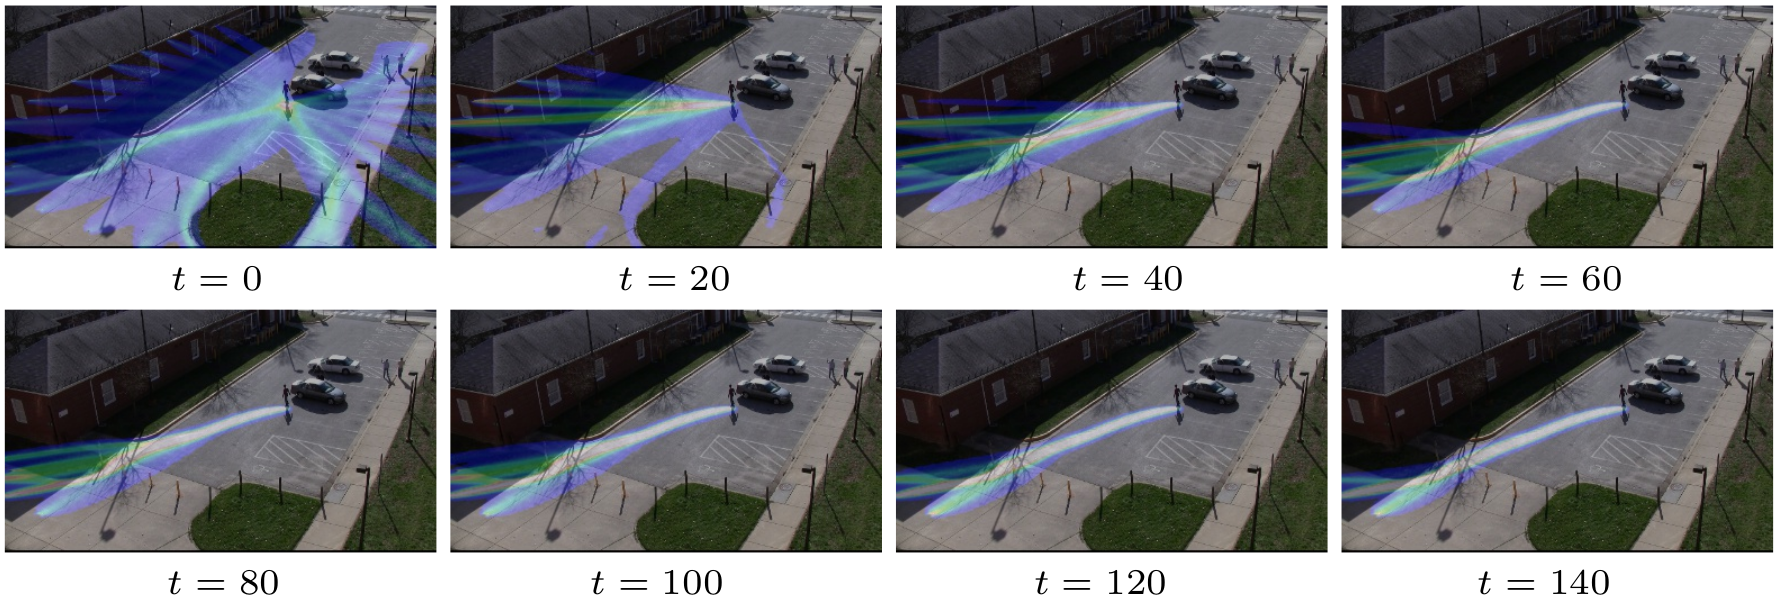
\includegraphics[scale=0.19]{Figures/ActivityForecasting.png}
			};
		\end{tikzpicture}
	\end{center}
	
	\vspace{-0.3cm}
	
	\tiny
	
	\cite{Kitani12} K. Kitani \emph{et al.}, ``Activity Forecasting'', ECCV, 2012
\end{frame}

\begin{frame}
	\frametitle{Advantages/Disadvantages}
	
	\Large
	
	\vspace{0.4cm}
	
	\underline{\textbf{Advantages}} \\
	
	\vspace{0.2cm}
	
	\begin{itemize}
		\item Knowledge transfer by using physical scene features
		\item Accurate and robust destination forecasting
	\end{itemize}
	
	\vspace{0.2cm}
	
	\underline{\textbf{Disadvantages}} \\
	
	\vspace{0.19cm}
	
	\begin{itemize}
		\item Prior knowledge of potential goals
		\item Space of possible motions is explicitly parametrised
		\item Applicability in dynamic environments? \\
			  \vspace{-0.2cm}
			  \begin{tabbing}
				  \hspace{0.3cm}
				  \large
				  $ \leadsto $ \emph{rescue or rapidly changing construction environment}
			  \end{tabbing}
	\end{itemize}
\end{frame}
